\section{Introduction}

Глава посвящена спектральному анализу решеток, в частности общей схеме спектрального анализа, базовым понятиям, теоретическим основам и возможным применениям для решения прикладных задач.

\section{References Review}

\begin{itemize}
    \item ~\cite{GDL} -- основная работа курса, глава которой содержит краткую обзорную информацию о методологии спектрального анализа решеток;
    \item ~\cite{SpectralMeshSurvey} -- наиболее полная обзорная статья, посвященная спектральному анализу решеток и стандартизации существующих подходов в данной области;
    \item ~\cite{SpectralMeshSurvey2} -- обзор существующих подходов к спектральному анализу решеток с математическим обоснованием (частично дублирует \cite{SpectralMeshSurvey});
    \item ~\cite{SpectralMeshSurveyCourse} -- семинар-практикум по спектральному анализу графов и решеток;
\end{itemize}

\section{Main Part}

Определим понятие треугольной решетки. 
\textit{Треугольная решетка} $\mathcal{M}$ -- ненаправленный граф с дополнительной структурой, то есть пара вида $(\mathcal{G}, \vect{P})$, где
	\begin{itemize} 
		\item $\mathcal{G} = (\mathcal{V}, \mathcal{E}) ~- $ граф, 
		\item $\mathcal{V} ~-$ множество вершин графа, 
		\item $\mathcal{E} \subset \mathcal{V} \times \mathcal{V} ~-$ множество ребер графа, 
		\item $\vect{P} = \left[ \vect{p}_1 \, \dots \vect{p}_n \right] \in \mathbb{R}^{n \times 3} ~- $ матрица трехмерных координат вершин решетки, то есть
		$\vect{p}_i = [x_i, y_i,z_i] ~-$ координаты вершины $i \in \mathcal{V}$. 
	\end{itemize}
Примером треугольной решетки может послужить триангуляция некоторой трехмерной фигуры.

\begin{figure}[!htb]
\center{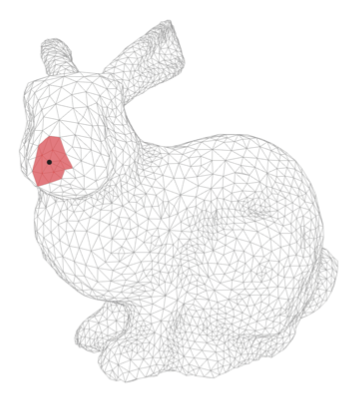
\includegraphics[width=5cm]{chapters/grigorev_s2/pictures/mesh_ex}}
\caption{Пример графовой решетки}
\end{figure}

\subsection{Лапласиан решетки}

Далее речь пойдет о спектральном анализе решеток. Большинство методов спектрального анализа имеют схожую схему, которая может быть обобщена следующим образом. В спектральном анализе предполагается $3$ основных этапа. На первом для заданной решетки определяется некоторый линейный оператор $\vect{M}$, элементы $M_{ij}$ которого соответствует информации о связи вершин $i$ и $j$. В частности $M_{ij}$ может нести информацию о смежности или относительном геометрическом расположении вершин $i$ и $j$ по отношению друг к другу. На втором этапе для определенного линейного оператора $\vect{M}$, заданного в матричном виде, вычисляются собственные числа и собственные вектора. В последствии производится анализ собственных чисел и собственных векторов оператора $\vect{M}$ с целью решение поставленной задачи.

Одним из вариантов выбора оператора $\vect{M}$ является комбинаторный лапласиан.
Комбинаторный лапласиан решетки $\mathcal{M} = (\mathcal{G}, \vect{P})$ полностью определяется ее графом $\mathcal{G} = (\mathcal{V}, \mathcal{E})$. Пусть $\vect{W} ~-$ матрица смежности графа $\mathcal{G}$, то есть 
		\begin{equation*}
		W_{ij} = 
		 \begin{cases}
   		1 &\text{если $(i,j) \in \mathcal{E}$,}\\
   		0 &\text{иначе.}
		 \end{cases}
		\end{equation*}
дополнительно вводится матрица $\vect{D}$ (\textit{degree matrix}) как 
		\begin{equation*}
		D_{ij} = 
		 \begin{cases}
   		d_i = |N(i)|&\text{если $i=j$,}\\
   		0 &\text{иначе,}
		 \end{cases}
		\end{equation*}
где $d_i ~-$ степень вершины $i \in \mathcal{V}$. Тогда комбинаторный лапласиан $\vect{K}$ (\textit{матрица Кирхгофа}) определяется как
		\begin{equation*}
		\vect{K} = \vect{D} -\vect{W}.
		\end{equation*}
Таким образом, комбинаторный лапласиан $\vect{K}$ содержит информацию о локальных свойствах решетки: смежности вершин и их степени. Геометрическая информация, о расположении вершин решетки, не используется для определения комбинаторного лапласиана.

Для комбинаторного лапласиана можно показать связь с оператором Лапласа-Бельтрами в случае риманова многообразия, в частности комбинаторный лапласиан является естественным обобщением данного оператора для решетки.
Оператор Лапласа-Бельтрами на римановом многообразии, действующий на гладкую функцию $\phi$: 
	$$\Delta(\phi) = \text{div}\, (\text{grad}(\phi)).$$
Пусть $\mathcal{G} = (\mathcal{V}, \mathcal{E}) ~-$ граф триангуляции данного риманова многообразия, а $f : \mathcal{V} \to \mathbb{R} ~- $ сужение функции $\phi$ на $\mathcal{V}$.
Определим ориентированную матрицу инцидентности $\vect{R} \in \mathbb{R}^{n \times m}$ графа $\mathcal{G}$, ориентация ребер которого задана произвольно:
	\begin{equation*}
		R_{ie} = 
		 \begin{cases}
   		-1 &\text{если $i \in \mathcal{V} ~-$ начальная вершина ребра $e \in \mathcal{E}$,}\\
   		+1 &\text{если $i \in \mathcal{V} ~-$ конечная вершина ребра $e \in \mathcal{E}$.}
		 \end{cases}
	\end{equation*}
Несложно заметить связь комбинаторного лапласиана и ориентированной матрицы инцидентности: $$\vect{K} = \vect{R} \vect{R}^T.$$
Тогда оператор $\vect{R}^T f : \hat{\mathcal{E}} \to \mathbb{R} $ действует на множестве направленных ребер $\hat{\mathcal{E}}: \,\, | \hat{\mathcal{E}}| = 2 |\mathcal{E}|$:
	$$(\vect{R}^T f)(e) = f(e^+) - f(e^-),$$
где $e^-, \, e^+ ~-$ начальная и конечная вершины ребра $e$ соответственно. 
	
Величина $(\vect{R}^T f)(e)$ может рассматривать как естественный аналог градиента функции $\phi$ на ребре $e$, тогда оператор $\vect{K} = \vect{R} \vect{R}^T $ соответствует дивергенции градиента. Таким образом, комбинаторный лапласиан решетки -- дискретный аналог оператора Лапласа-Бельтрами. При измельчении размера триангуляции в пределе комбинаторный лапласиан соответсвует непрерывному оператору Лапласа-Бельтрами.

\subsection{Спектр лапласиана}

Свойства комбинаторного лапласиана позволяют в некоторой степени описать его спектр. В частности для комбинаторного лапласиана выполнена спектральная теорема, поскольку лапласиан является симметричной положительно полуопределенной матрицей. \medskip

\textbf{Cпектральная теорема}

Пусть $\vect{S} \in \mathbb{R}^{n \times n} ~- $ действительнозначная симметричная матрица, тогда ее спектральное разложение:
$$\vect{S} = \vect{V}  \bm{\Lambda} \vect{V}^T = \sum \lambda_i \vect{v}_i \vect{v}_i^T,$$ 
где $\vect{V} = [\vect{v}_1 \, \dots \, \vect{v}_n] ~- $  матрица, составленная из собственных векторов матрицы $\vect{S}$, $ \bm{\Lambda} ~-$ диагональная матрица из собственных значений матрицы $\vect{S}$. Причем собственные значения действительный, а собственные вектора ортогональны.

Из положительной полуопределенности комбинаторного лапласиана следует, что его собственные значения неотрицательны. В частности комбинаторный лапласиан вырожден, его наименьшее собственное значение равно $0$, кратность данного собственного значения равна числу компонент связности графа, то есть для решетки кратность в общем случае равна $1$. Собственные вектора лапласиана ортогональны.

\begin{figure}[!htb]
\center{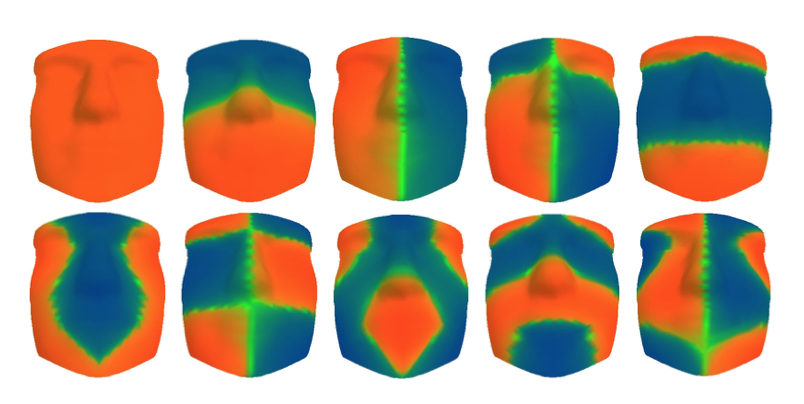
\includegraphics[width=10cm]{chapters/grigorev_s2/pictures/face_mesh}}
\caption{Визуализация первых $10$ собственных векторов лапласиана решетки лица}
\end{figure}

\subsection{Спектральное преобразование}

Ортогональность собственных векторов комбинаторного лапласиана позволяет рассматривать их как аналог Фурье базиса.  Обратное дискретное преобразование Фурье соответствует разложению исходного сигнала по ортогональному базису 
	$$\vect{x} = \sum \limits _{k=0}^{n-1} y_k \bm{\psi}_k = \bm{\Psi} \vect{y},$$ 
где $\{ \bm{\psi}_k\}_{k=0}^{n-1} ~- $ базис Фурье, $\vect{x} ~- $ исходный сигнал, $\vect{y} ~- $ его Фурье образ.
Собственные вектора $\vect{v}_1 \, \dots \, \vect{v}_n$ лапласиана $\vect{K}$ образуют аналог базиса Фурье, соответствующие им собственные значения рассматриваются как частоты.
На практике собственные вектора подобны гармоникам.
Тогда может быть введено спектральное преобразование, подобное дискретному преобразованию Фурье, которое определяется через собственные вектора $\vect{v}_1 \, \dots \, \vect{v}_n$  \, ($\lambda_1 \le \dots \le \lambda_n$) лапласиана $K$:
	$$\vect{Y} = \vect{V}^T \vect{X},$$
где $\vect{V} = [\vect{v}_1 \, \dots \, \vect{v}_n]$, $\vect{X} \in \mathbb{R}^{n \times 3} ~- $ координатный сигнал на решетке, $\vect{Y} ~- $ образ.

Данное спектральное преобразование имеет общие свойства с преобразованием Фурье, из чего вытекают схожие применения, например, фильтрация сигнала на решетке.
В частности фильтрация координатного сигнала $x: \mathcal{V} \to \mathbb{R}^3$, $x(i)=\vect{p}_i$ на решетке $\mathcal{M}=(\mathcal{V}, \mathcal{E}, \vect{P})$ состоит в последовательном применении DFT-подобного спектрального преобразования, оператора фильтрации и обратного спектрального преобразования.
\begin{figure}[!htb]
\center{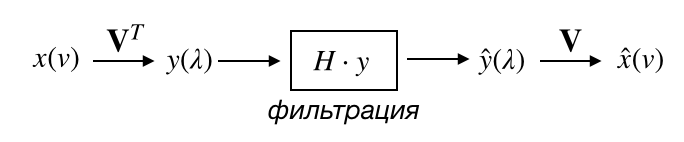
\includegraphics[width=10cm]{chapters/grigorev_s2/pictures/filtration_scheme}}
\caption{Схема фильтрации координатного сигнала}
\end{figure}
На практике зачастую выбирается фильтр нижних частот, пропускающий лишь компоненты, отвечающие меньшим собственным значениям лапласиана $\vect{K}$, которые в данном случае рассматриваются в качестве частот.
Частным случаем спектральной фильтрации является спектральная компрессия -- фильтрация с идеальным фильтром низких частот, то есть пропускающим лишь $k$ наименьших частот спектра.

\begin{figure}[!htb]
\center{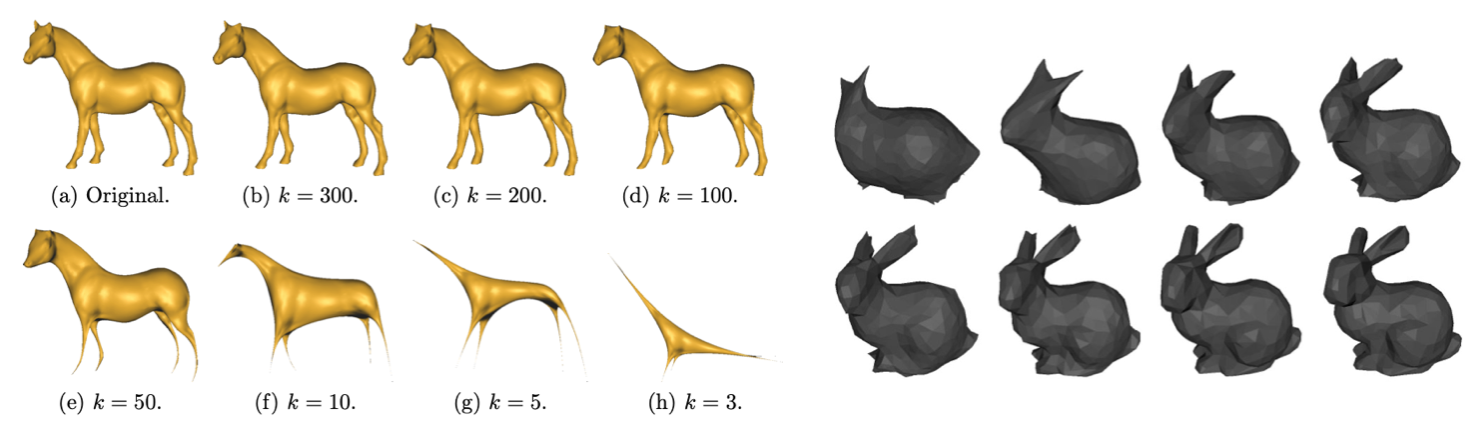
\includegraphics[width=14cm]{chapters/grigorev_s2/pictures/rabbit_horse_mesh}}
\caption{Примеры восстановления решеток с применением спектральной компрессии}
\end{figure}

\subsection{Cпектральный дескриптор}

Лапласиан $\vect{K}$ решетки описывает локальную информацию о ее структуре: смежность вершин и их степень, однако согласно спектральной теории графов собственные значения и собственные векторы лапласиана $\vect{K}$ несут значимую (достаточно полную) глобальную информацию о решетке.  В связи с этим во многих практических приложениях для решения задач используется не сам комбинаторный лапласиан, а спектральный дескриптор, определяющийся через собственные значения и собственные векторы комбинаторного лапласиана и представляющий собой эмбеддинг, сохраняющий полную информацию о лапласиане.
Для спектрального разложения $\vect{K} = \vect{V}  \bm{\Lambda} \vect{V}^T $ лапласиана $\vect{K}$ заданной решетки $\mathcal{M}$ спектральный дескриптор определяется как:
	$$\vect{W} = \vect{V} \bm{\Lambda}^{1/2},$$
спектральный дескриптор полностью описывает лапласиан $\vect{K} = \vect{W} \vect{W}^T$.

Использование полного спектрального дескриптора $\vect{W}$ осложняется его высокой размерность, в связи с этим требуется производить снижение размерности дескриптора для его эффективного применения.
Оптимальный метод снижения размерности спектрального дескриптора $\vect{W}$ описывается следующей теоремой.\medskip

\textbf{Теорема (\textit{Eckart-Young})}
\begin{itemize}
\item $\vect{S} \in \mathbb{R}^{n \times n} ~- $ действительнозначная симметричная положительно полуопределенная матрица, ее спектральное разложение $\vect{S} = \vect{V}  \bm{\Lambda} \vect{V}^T $. Собственные значения на диагонали матрицы $\bm{\Lambda}$ расположены по убыванию. 
\item $\vect{W} = \vect{V} \bm{\Lambda}^{1/2} ~-$ матрица собственных векторов, масштабированных на корень соответствующих собственных значений.
\item $\vect{W}_{(k)} \in \mathbb{R}^{n \times k} ~- $ усеченная матрица $\vect{W}$, состоящая из $k$ первых столбцов $\vect{W}$.
\item $\vect{W}_{(k)} \vect{W}_{(k)}^T ~-$ лучшая в терминах нормы Фробениуса аппроксимация ранга $k$ для матрицы $\vect{S}$:
$$\vect{W}_{(k)} = \arg \min \limits _{\substack{\vect{U} \in \mathbb{R}^{n \times k} \\ \text{rank}(\vect{U})=k}} \| \vect{S} - \vect{U} \vect{U}^T \|$$
\end{itemize}


Таким образом, уменьшение размерности спектрального дескриптора $\vect{W}$ выбором подматрицы $\vect{W}_{(k)}$, отвечающей $k$ наибольшим собственным значениям лапласиана $K$, оптимально с точки зрения сохранения информации.

\section{Questions To Discussion}
\begin{enumerate}
\item Чем заменить матрицу смежности в определении комбинаторного лапласиана, чтобы он учитывал геометрическую структуру (координаты) решетки?
\item Почему описанный лапласиан называется комбинаторным?
\item Как определить критерий выбора параметра $k$ (число частот после фильтрации) в спектральной компрессии? 
\item Чему равно наименьшее собственное значение и соответствующий собственный вектор комбинаторного лапласиана $\vect{K}$? Почему визуализация данного собственного значения отлична от остальных?
\end{enumerate}